\chapter{Maxwell Equations, Covariance, and Electromagnetic Waves}

We begin where the previous lecture left off. We already know how electric and magnetic fields act on charged particles; the Lorentz force law tells us that part of the story. The missing half is the reverse question: what determines the fields themselves, and how do charges and currents generate them? In this lecture Leonard Susskind answers that question in a deliberately relativistic way. Maxwell's equations are not presented merely as a list to memorize, but as laws to be written in tensor form, checked component by component, and then used to derive the existence of light waves. Throughout we work in units with \(c=1\). These notes follow Leonard Susskind closely and are curated by LazyingArt LLC.

\section{From the Lorentz Force to the Missing Field Equations}

The lecture opens by looking backward. Electric and magnetic fields push charged particles around, and the force is proportional to the charge because an uncharged particle does not feel the electromagnetic field at all. In ordinary three-vector language the law is
\begin{align}
\mathbf F = q\bigl(\mathbf E + \mathbf v \times \mathbf B\bigr).
\end{align}
This is the familiar half of electromagnetism: fields act on matter.

\begin{figure}[h]
\centering

\includegraphics[width=0.58\textwidth]{lecture_58_figure_02.png}
\caption{Lorentz force rewritten in field-tensor notation.}
\end{figure}

The board then pivots schematically toward covariant notation. As written on the board, that second line is incomplete; the clean covariant form is
\begin{align}
f^\mu = q\,F^\mu{}_{\nu}\,u^\nu.
\end{align}
Here \(f^\mu\) is the four-force, \(u^\nu\) is the four-velocity, and \(F^{\mu\nu}\) is the antisymmetric electromagnetic field tensor that we will construct shortly. The point of the reminder is not just notation. Written this way, the force law is manifestly the same in every inertial frame.

What is missing, then, is not the dynamics of a charged particle in a given field. What is missing is the dynamics of the field itself. What decides whether there is an electric field here, a magnetic field there, or an electromagnetic wave moving through empty space? Those are the equations we now need, and those equations are Maxwell's equations.

\section{Why Charges Must Affect Fields}

Susskind does not introduce Maxwell's equations as an abstract completion of formalism. He motivates them physically. If a point charge sits somewhere in space, it creates an electric field that spreads outward from it. If charges move through a wire, their motion creates a magnetic field that circulates around the wire. So already, even before we write equations, we know the rough empirical content: charges and currents generate fields.

But the lecture quickly sharpens the issue. Suppose we suddenly move a point charge. The field cannot rearrange itself instantaneously throughout all space. A distant observer is not allowed to learn about the change before a light signal could have arrived. Thus the rearrangement of the field must spread outward in time. If we move the charge back and forth, that rearrangement becomes a propagating electromagnetic wave. The same reasoning applies to a current in a wire: reverse the current, and the change in the magnetic field must propagate outward causally, again as an electromagnetic disturbance.

\subsection{Question \& Answer}

\paragraph{Question.} Why must charged matter act back on the electromagnetic field?

\paragraph{Answer.} Because otherwise energy conservation would fail. An electromagnetic wave can strike a charged particle and give it energy and momentum. If that process is possible, then the reverse influence must also be possible: charged matter must be able to extract energy from the field and alter it. The statement is sometimes framed as action and reaction, but the lecture puts the sharper point on conservation laws. Once the field can do work on matter, matter must be able to affect the field.

This is the physical bridge to Maxwell's equations. They must not merely describe static sources; they must also describe the causal propagation of changes in the field.

\section{Wave Review and Vector Calculus}

Before writing Maxwell's equations in earnest, the lecture pauses for mathematical review. We first recall the simple relativistic wave equation for a scalar field \(\phi\):
\begin{align}
\partial_\mu \partial^\mu \phi = 0.
\end{align}
With the usual sign choice implicit in the lecture, this means
\begin{align}
\partial_t^2 \phi - \partial_x^2 \phi - \partial_y^2 \phi - \partial_z^2 \phi = 0.
\end{align}
If the wave moves only along the \(z\)-axis, then \(\phi\) depends on \(z\) and \(t\) but not on \(x\) or \(y\), so the equation reduces to
\begin{align}
\partial_t^2 \phi - \partial_z^2 \phi = 0.
\end{align}

\begin{figure}[h]
\centering

\includegraphics[width=0.56\textwidth]{lecture_58_figure_04.png}
\caption{One-dimensional wave equation for \(\phi\).}
\end{figure}

This equation has the two basic traveling-wave solutions
\begin{align}
\phi = f(z-t), \qquad \phi = g(z+t),
\end{align}
representing right-moving and left-moving profiles. A particularly useful example is the sinusoidal wave
\begin{align}
\phi(z,t) = \cos\!\bigl(k(z-t)\bigr),
\end{align}
where \(k\) is the wave number. Large \(k\) means short wavelength; small \(k\) means long wavelength. This is the prototype that will later reappear for the electric and magnetic fields themselves.

The lecture then reviews the bits of vector calculus that Maxwell's equations use. For ordinary three-vectors,
\begin{align}
\mathbf a \cdot \mathbf b &= a_x b_x + a_y b_y + a_z b_z,\\
(\mathbf a \times \mathbf b)_x &= a_y b_z - a_z b_y,
\end{align}
with the \(y\)- and \(z\)-components obtained by cyclic permutation. For a vector field \(\mathbf A\),
\begin{align}
\nabla \cdot \mathbf A &= \partial_x A_x + \partial_y A_y + \partial_z A_z,\\
(\nabla \times \mathbf A)_x &= \partial_y A_z - \partial_z A_y,
\end{align}
again with cyclic permutations for the other components.

The lecture keeps the geometric meaning in view. Divergence measures the extent to which a field seems to emanate from somewhere. Curl measures the extent to which it circulates around something. An electric field radiating from a charge is the model of divergence. A magnetic field winding around a wire is the model of curl.

\section{Vacuum Maxwell Equations and the Relativity Puzzle}

Now we write the source-free Maxwell equations, in the order used in the lecture:
\begin{align}
\nabla \times \mathbf E &= -\,\partial_t \mathbf B,\\
\nabla \cdot \mathbf B &= 0,\\
\nabla \times \mathbf B &= \partial_t \mathbf E,\\
\nabla \cdot \mathbf E &= 0.
\end{align}
These are the vacuum Maxwell equations. They describe electric and magnetic fields in the absence of charge density and current density.

At once one sees a certain symmetry. The equations involving curls almost turn into each other under \(\mathbf E \leftrightarrow \mathbf B\), but not quite: there is an essential sign difference. One also sees an asymmetry between the divergence equations. The electric field can later have a source \(\rho\); the magnetic field has no analogous source term in this lecture, and so \(\nabla \cdot \mathbf B = 0\).

For the moment Susskind deliberately postpones \(\rho\) and \(\mathbf J\). He mentions that they will reappear, but he brackets them off so that the vacuum structure can be seen without distraction.

\subsection{Question \& Answer}

\paragraph{Question.} How can Maxwell's equations be the same in every frame if they imply the same light speed in every frame?

\paragraph{Answer.} That is exactly the relativistic puzzle. If Maxwell's equations are the laws of light, and if those laws are the same in every inertial frame, then every inertial frame must extract the same light speed from them. The resolution is not to modify the equations frame by frame, but to rewrite them in terms of objects---vectors and tensors---whose transformation properties are already known. Once the equations are manifestly covariant, the constancy of the speed of light is not an accident. It is built into the structure of the laws.

This is why the lecture now turns to the field tensor. The real payoff is not elegance for its own sake, but manifest Lorentz invariance.

\section{The Electromagnetic Field Tensor}

The electric and magnetic fields combine into a single antisymmetric \(4\times 4\) tensor. In the lecture the time coordinate is placed first, so the row and column order is \(t,x,y,z\). The visible part of the board already fixes the sign pattern of the electric entries.

\begin{figure}[h]
\centering

\includegraphics[width=0.54\textwidth]{lecture_58_figure_03.png}
\caption{Electromagnetic field tensor with electric-field entries.}
\end{figure}

With the lecture's sign convention we write
\begin{align}
F^{\mu\nu}=
\begin{pmatrix}
0 & -E_x & -E_y & -E_z\\
E_x & 0 & -B_z & B_y\\
E_y & B_z & 0 & -B_x\\
E_z & -B_y & B_x & 0
\end{pmatrix}.
\end{align}
The diagonal vanishes because the tensor is antisymmetric, and the entries below the diagonal are the negatives of those above it.

The lecture then introduces a second antisymmetric tensor, the dual tensor \(\tilde F^{\mu\nu}\). We need only the rule that produces it. With the sign convention fixed above, the lecture's replacement rule is
\begin{align}
\mathbf E \mapsto -\,\mathbf B, \qquad \mathbf B \mapsto \mathbf E,
\end{align}
together with the same antisymmetry. Susskind corrects himself verbally while discussing the signs, so it is better here to fix one convention and use it consistently than to overdevelop the dual tensor beyond what the lecture needs.

The covariant vacuum Maxwell equations are then guessed almost by necessity. Maxwell's equations involve first derivatives and should leave one free index, so the natural candidate is
\begin{align}
\partial_\mu F^{\mu\nu} &= 0,\\
\partial_\mu \tilde F^{\mu\nu} &= 0.
\end{align}
There are four equations in the first line, one for each value of \(\nu\), and four in the second.

It is worth checking that this really reproduces the familiar equations. For the time component,
\begin{align}
\partial_\mu F^{\mu t}
&= \partial_t F^{tt} + \partial_x F^{xt} + \partial_y F^{yt} + \partial_z F^{zt}\\
&= \partial_x E_x + \partial_y E_y + \partial_z E_z\\
&= \nabla \cdot \mathbf E.
\end{align}
Thus \(\partial_\mu F^{\mu t}=0\) is exactly \(\nabla \cdot \mathbf E=0\).

A spatial component works the same way. Taking \(\nu=z\),
\begin{align}
\partial_\mu F^{\mu z}
&= \partial_t F^{tz} + \partial_x F^{xz} + \partial_y F^{yz} + \partial_z F^{zz}\\
&= -\,\partial_t E_z + \partial_x B_y - \partial_y B_x\\
&= -\,\partial_t E_z + (\nabla \times \mathbf B)_z.
\end{align}
So \(\partial_\mu F^{\mu z}=0\) is precisely the \(z\)-component of
\begin{align}
\nabla \times \mathbf B = \partial_t \mathbf E.
\end{align}
The other spatial components are analogous, and the equation with \(\tilde F^{\mu\nu}\) packages \(\nabla\cdot \mathbf B=0\) together with \(\nabla\times \mathbf E = -\,\partial_t \mathbf B\).

This is the formal center of the lecture. Maxwell's equations are now written as tensor equations, so their invariance from frame to frame is visible at a glance.

\section{From Maxwell to Electromagnetic Waves}

Once covariance is established, the lecture immediately asks what the equations actually say. The answer is that they admit wave solutions. To see this, start from
\begin{align}
\nabla \times \mathbf B = \partial_t \mathbf E
\end{align}
and differentiate once more with respect to time:
\begin{align}
\partial_t^2 \mathbf E = \nabla \times \partial_t \mathbf B.
\end{align}
Now use the other curl equation,
\begin{align}
\partial_t \mathbf B = -\,\nabla \times \mathbf E,
\end{align}
to eliminate \(\mathbf B\). This gives
\begin{align}
\partial_t^2 \mathbf E = -\,\nabla \times (\nabla \times \mathbf E).
\end{align}

The board algebra then expands the \(x\)-component in detail. The clean summary of that algebra is
\begin{align}
\partial_t^2 E_x
&= -\bigl(\nabla \times (\nabla \times \mathbf E)\bigr)_x\\
&= -\,\partial_x(\nabla \cdot \mathbf E)
   + \partial_x^2 E_x + \partial_y^2 E_x + \partial_z^2 E_x.
\end{align}
In vacuum, \(\nabla \cdot \mathbf E = 0\), so we arrive at
\begin{align}
\partial_t^2 E_x - \partial_x^2 E_x - \partial_y^2 E_x - \partial_z^2 E_x = 0.
\end{align}
Thus a component of the electric field satisfies the same wave equation as the scalar field reviewed earlier. The lecture's payoff is immediate: electromagnetic fields themselves can propagate as waves.

A particularly simple example is a wave moving along the \(z\)-axis:
\begin{align}
E_x(z,t) = \cos(z-t), \qquad E_y = 0.
\end{align}
This is a right-moving wave in the lecture's \(c=1\) units. It is also a polarized wave: the electric field has been chosen to lie along the \(x\)-direction. With the sign convention fixed above, one matching magnetic field is
\begin{align}
B_y(z,t) = \cos(z-t), \qquad B_x = B_z = 0,
\end{align}
which indeed satisfies \(\nabla \times \mathbf E = -\,\partial_t \mathbf B\).

\subsection{Question \& Answer}

\paragraph{Question.} Why must the electromagnetic wave be transverse?

\paragraph{Answer.} Because the divergence and curl equations leave no room for a propagating longitudinal part. For a wave depending only on \(z\) and \(t\),
\begin{align}
\nabla \cdot \mathbf E
= \partial_x E_x + \partial_y E_y + \partial_z E_z
= \partial_z E_z.
\end{align}
In vacuum this must vanish, so
\begin{align}
\partial_z E_z = 0.
\end{align}
Hence the \(z\)-component of the electric field can at most be a constant. A constant field is not part of the wave profile, so the wave part of \(E_z\) vanishes.

Next, since \(E_x(z,t)\) is nonzero while \(E_y\) and the wave part of \(E_z\) are zero, the only nonvanishing component of \(\nabla \times \mathbf E\) lies along \(y\). But \(\nabla \times \mathbf E = -\,\partial_t \mathbf B\), so the magnetic field itself must lie along \(y\). Therefore
\begin{align}
\mathbf E \perp \hat z, \qquad \mathbf B \perp \hat z, \qquad \mathbf E \perp \mathbf B.
\end{align}
That is the transversality of electromagnetic radiation.

\begin{remark}
The next frame is kept because it preserves the board geometry of the wave, even though its subtitle metadata is mismatched. Its value here is visual rather than timestamp evidence.
\end{remark}

\begin{figure}[h]
\centering

\includegraphics[width=0.48\textwidth]{lecture_58_figure_05.png}
\caption{Board sketch of a transverse wave propagating along \(z\).}
\end{figure}

\begin{figure}[h]
\centering
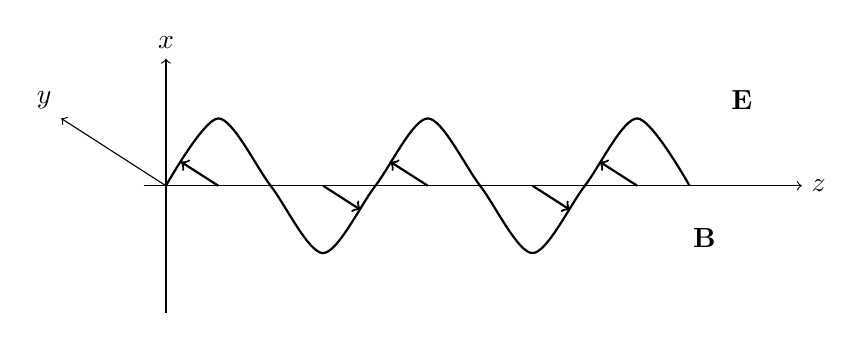
\begin{tikzpicture}[scale=0.95]
\draw[->] (-0.3,0) -- (8.5,0) node[right] {$z$};
\draw[->] (0,-1.7) -- (0,1.7) node[above] {$x$};
\draw[->] (0,0) -- (-1.4,0.9) node[above left] {$y$};

\draw[thick] plot[smooth] coordinates {
(0.0,0.0)
(0.7,0.9)
(1.4,0.0)
(2.1,-0.9)
(2.8,0.0)
(3.5,0.9)
(4.2,0.0)
(4.9,-0.9)
(5.6,0.0)
(6.3,0.9)
(7.0,0.0)
};

\draw[->,thick] (0.7,0.0) -- (0.2,0.32);
\draw[->,thick] (2.1,0.0) -- (2.6,-0.32);
\draw[->,thick] (3.5,0.0) -- (3.0,0.32);
\draw[->,thick] (4.9,0.0) -- (5.4,-0.32);
\draw[->,thick] (6.3,0.0) -- (5.8,0.32);

\node at (7.7,1.15) {$\mathbf E$};
\node at (7.2,-0.7) {$\mathbf B$};
\end{tikzpicture}
\caption{A clean reconstruction of the transverse electromagnetic-wave geometry: propagation along \(z\), electric field along \(x\), magnetic field along \(y\).}
\end{figure}

So the lecture reaches its physical climax: Maxwell's equations imply electromagnetic waves, and those waves move with speed \(1\), namely the speed of light in the chosen units.

\section{Restoring Sources: Charge, Current, Continuity, and Covariance}

Having studied the clean vacuum case, we now restore the charge and current that were postponed earlier. The sourced Maxwell equations are
\begin{align}
\nabla \cdot \mathbf E &= \rho,\\
\nabla \cdot \mathbf B &= 0,\\
\nabla \times \mathbf E &= -\,\partial_t \mathbf B,\\
\nabla \times \mathbf B &= \partial_t \mathbf E + \mathbf J.
\end{align}

The charge density \(\rho\) is defined as charge per unit volume:
\begin{align}
\rho = \frac{dQ}{dV}.
\end{align}
In a continuum description the charge in a region \(V\) is therefore
\begin{align}
Q_V = \int_V \rho\,dV.
\end{align}
The lecture emphasizes that \(\rho\) may depend on position and on time. Charge may move from place to place, so local density can change, but not arbitrarily: charge is conserved.

To express local transport we introduce the current density \(\mathbf J\). If \(d\boldsymbol{\sigma}\) is the oriented surface element vector, then the charge per unit time flowing through that surface element is
\begin{align}
\frac{dQ}{dt} = \mathbf J \cdot d\boldsymbol{\sigma}.
\end{align}
This is why current is a vector. Its magnitude is charge per unit area per unit time, and its direction is the direction of flow.

Now fix a region \(V\) with outward-pointing boundary element \(d\boldsymbol{\sigma}\). If charge flows outward through the boundary, the charge inside must decrease. Thus
\begin{align}
\frac{dQ_V}{dt} = -\oint_{\partial V} \mathbf J \cdot d\boldsymbol{\sigma}.
\end{align}
But \(Q_V=\int_V \rho\,dV\), so
\begin{align}
\int_V \partial_t \rho\,dV = -\oint_{\partial V} \mathbf J \cdot d\boldsymbol{\sigma}.
\end{align}
Now apply Gauss's theorem,
\begin{align}
\oint_{\partial V} \mathbf A \cdot d\boldsymbol{\sigma}
= \int_V (\nabla \cdot \mathbf A)\,dV,
\end{align}
to the current field \(\mathbf J\). Then
\begin{align}
\int_V \partial_t \rho\,dV
= -\int_V (\nabla \cdot \mathbf J)\,dV.
\end{align}
Since this holds for every volume \(V\), the integrands must agree:
\begin{align}
\partial_t \rho + \nabla \cdot \mathbf J = 0.
\end{align}
This is the continuity equation, the local statement of charge conservation.

The relativistic packaging is now obvious. The four quantities \(\rho, J_x, J_y, J_z\) form the four-current
\begin{align}
J^\mu = (\rho, J_x, J_y, J_z),
\end{align}
and the continuity equation becomes
\begin{align}
\partial_\mu J^\mu = 0.
\end{align}

At the same time, the sourced Maxwell equations take the compact covariant form
\begin{align}
\partial_\mu F^{\mu\nu} = J^\nu.
\end{align}
For \(\nu=t\), the right-hand side is \(J^t=\rho\), and we recover
\begin{align}
\nabla \cdot \mathbf E = \rho.
\end{align}
For spatial \(\nu\), we recover
\begin{align}
\nabla \times \mathbf B = \partial_t \mathbf E + \mathbf J.
\end{align}
The other half of Maxwell's equations remains
\begin{align}
\partial_\mu \tilde F^{\mu\nu} = 0.
\end{align}

So the return of sources does not spoil covariance. On the contrary, it completes it. Charges and currents themselves enter as a four-vector, and the sourced field equations remain tensor equations.

\section{Summary}

The lecture has a very definite arc. We start from the Lorentz force law and identify the missing half of electromagnetism: not how fields act on matter, but how matter determines fields. Maxwell's equations answer that question. In vacuum they can be written as the covariant equations \(\partial_\mu F^{\mu\nu}=0\) and \(\partial_\mu \tilde F^{\mu\nu}=0\), and from them one derives wave equations for the field components themselves. A plane-wave solution then shows that electromagnetic radiation is transverse and polarized, with \(\mathbf E\), \(\mathbf B\), and the propagation direction mutually perpendicular.

Finally, when charges and currents are restored, the continuity equation and the four-current \(J^\mu\) allow the sourced equations to be written as \(\partial_\mu F^{\mu\nu}=J^\nu\). That is the closing message of the lecture: the laws of electromagnetism can be written in tensor form, so they are the same in every inertial frame, and because those same laws imply waves moving with speed \(c\), light moves with the same speed in every inertial frame.